% !Mode:: "TeX:UTF-8"

% 请使用 XeLaTeX 编译本文.
%\documentclass[forprint]{HENU-Bachelor-LaTeX}
\documentclass{HENU-Bachelor-LaTeX}
% 选项 forprint: 交付打印时使用, 避免彩色链接字迹打印偏淡. 
% 注意:一般要求新的章开始于新的奇数页,所以在合适的地方已经设置好空白页,直接双面打印即可!无需更多设置。

\begin{document}

% 下面的内容主要自动产生封面, 按要求修改内容即可.

%\miji{ }                   % 密级, 没有就空着.
\Year{2023}                 % 毕业年份
%-------------------------中文封面 --------------------------------------%
\title{河南大学毕业论文 \LaTeX 模板}            % 题目
\author{Icey}                     % 姓名
\StudentNumber{\href{https://www.icey.one}{Icey One}}        % 学号
\Cschoolname{数学与统计学院}        % 学院名
\Cmajor{数学与应用数学}             % 专业中文名
\Ctutorname{导师名}                 % 指导教师姓名
\Ctutortitle{教授}                  % 指导老师职称
\date{2023 年 5 月 6 日}          % 日期, 要注意和英文日期一致!!

%\pdfbookmark[0]{封面}{title}         % 封面页加到 pdf 书签
\maketitle
%\pagestyle{empty}
\frontmatter
\pagenumbering{Roman}            % 正文之前的页码用大写罗马字母编号.
%----------- 前言 Frontmatte -------%
% !Mode:: "TeX:UTF-8"

%====此部分需要自行填写: (1) 中文摘要及关键词 (2) 英文摘要及关键词===%

%%---------------英文封面-------------%%

%\thispagestyle{empty}
%\renewcommand{\baselinestretch}{1.5}  %下文的行距
%\vspace*{0.5cm}
%\begin{center}
%  {\Large \bf BACHELOR'S DEGREE THESIS \\[1ex] OF HENAN UNIVERSITY }
%\end{center}
%
%\vspace{2.5cm}
%
%\begin{center}{\zihao{2}
%  \the\Etitle \par}
%\end{center}
%
%\vfill
%
%\begin{center}
%  \zihao{4}
%  \begin{tabular}{ r l }
%    School:         & {\sc  \the\Eschoolname} \\
%    Major:          & {\sc  \the\Emajor}      \\
%    Candidate:      & {\sc  \the\Eauthor}     \\
%    Supervisor:     & {\sc  \the\Esupervisor}
%  \end{tabular}
%
%  \vspace*{2cm}
%
%  \begin{center}
%    \ifprint % 文档打印, 使用黑白校徽.
%    \includegraphics[height=4cm]{hedalogo.pdf}       %%  黑白的.
%    \else
%    \includegraphics[height=4cm]{hedalogo.pdf} %%  彩色的.
%    \fi
%\end{center}
%
%
%\zihao{-2}
%\the\Schoolname\\
%{\sc Henan University}
%
%\vspace*{1.0cm}
%
%\the\Edate
%
%\end{center}

%%---------------郑重声明 (本科不需要)----------------------------%
%\newpage
%\vspace*{20pt}
%\begin{center}{\ziju{0.8}\textbf{\songti\zihao{2} 郑重声明}}\end{center}
%\par\vspace*{30pt}
%\renewcommand{\baselinestretch}{2}
%
%{\zihao{4}%
%
%本人呈交的学位论文, 是在导师的指导下, 独立进行研究工作所取得的成果, 所有数据、图片资料真实可靠. 
%尽我所知, 除文中已经注明引用的内容外, 本学位论文的研究成果不包含他人享有著作权的内容. 
%对本论文所涉及的研究工作做出贡献的其他个人和集体, 均已在文中以明确的方式标明. 本学位论文的知识产权归属于培养单位.\\[2cm]
%
%\hspace*{1cm}本人签名: $\underline{\hspace{3.5cm}}$
%\hspace{2cm}日期: $\underline{\hspace{3.5cm}}$\hfill\par}
%%------------------------------------------------------------------------------
%\baselineskip=23pt  % 正文行距为 23 磅
%%------------------------------------------------------------------------------
%



%%===========中文摘要起始===================%
\begin{cnabstract}
\thispagestyle{empty}
此为河南大学本科生毕业论文 \LaTeX 模板, 修改自 \href{https://github.com/davidgao666/HedaBachelorTemplate}{HedaBachelorTemplate}. 几乎重写了整个模板, 修改了陈年 BUG, 增加了亿点细节.

查看更新请去 \href{https://github.com/Icey-u/HENU-Bachelor-LaTeX-Template}{HENU-Bachelor-LaTeX-Template}
\end{cnabstract}
\par
\vspace*{2em} %%产生空行

%%-------------关键词----------------------%%
%%%-- 在下面的大括号中写入的关键词。注意: 每个关键词之间用“;”分开,最后一个关键词不打标点符号
\cnkeywords{\LaTeX; 模板; 河大; 毕业论文}
%===========中文摘要结束===================%

\cleardoublepage % 空白页

%=============英文摘要起始=====================%

\begin{enabstract}
  This is the \LaTeX template of Henan University, modified form \href{https://github.com/davidgao666/HedaBachelorTemplate}{HedaBachelorTemplate}. Almost rewrote the entire template, modified many old bugs, and added lots of details.

  Scr: \href{https://github.com/Icey-u/HENU-Bachelor-LaTeX-Template}{HENU-Bachelor-LaTeX-Template}
\end{enabstract}
\par
\vspace*{2em}

%%------------ Key words --------------------%%
\enkeywords{\LaTeX, Template; HENU; Paper}
%=============英文摘要结束=====================%
\thispagestyle{empty}
\cleardoublepage % 空白页


    % 加入中英文摘要.中英文摘要请打开frontmatter.tex文档撰写。

\thispagestyle{empty}
%\pdfbookmark[0]{目录}{toc}
\tableofcontents
\thispagestyle{empty}

\mainmatter % 以下正文
%------------正文 Mainmatter----------%
%\newpage
\chapter{绪论}
文档源地址 \href{https://github.com/Icey-u/HENU-Bachelor-LaTeX-Template}{HENU-Bachelor-LaTeX-Template}, 请自行查看是否更新. 

对于理工科来说, \LaTeX 很好的解决了公式排版的问题, 能够让大家把精力放在论文内容而非格式上. 

点名批评河南某大学数学院明明学过 \LaTeX, 却在要写毕业论文时只提供了 Word 模板选项, 因为我不会使用 Word, 所以自己用 \LaTeX 造了个轮子.

本文档为河南大学本科毕业论文 \LaTeX 模板, 适用于 2023 年数学院《毕业论文格式要求》. 下面介绍一下使用方法和其他内容.
\section{使用方法}
主文档使用 \hologo{XeLaTeX} 编译, 若要使用参考文献, 则使用 \hologo{XeLaTeX} => \hologo{BibTeX} => \hologo{XeLaTeX} 编译. 每次目录变动均需编译两次 (\hologo{XeLaTeX}*2)才可.

如果你还不太熟悉 \LaTeX, 那么我建议看 \href{https://liam.page/2014/09/08/latex-introduction/}{一份其实很短的 LaTeX 入门文档} 以及 \href{https://www.ctan.org/pkg/lshort-zh-cn}{lshort-zh-cn}.

下面开始介绍本文档使用方法, 本模板存在两种文档类型;
\begin{lstlisting}
    \documentclass{HENU-Bachelor-laTeX}           % 彩色版
    \documentclass[forprint]{HENU=Bachelor-LaTeX} % 打印版
\end{lstlisting}
其中彩色版有超链接突出显示, 而打印版隐藏了超链接颜色, 建议在交付论文时使用打印版, 避免打印字迹偏淡. 
\chapter{字体设置}
本文档已按照《本科生毕业论文格式规范》设定相应字体\footnote{请确保已安装相关字体}, 如果您需要进行一些改动, 下面是一个很好的例子.    
\begin{lstlisting}
    \songti{我想要正文是宋体}
    \heiti{标题是黑体}
    \fangsong{页眉是仿宋}
    \kaishu{参考文献是楷书}
\end{lstlisting}
\songti{我想要正文是宋体}, \heiti{标题是黑体}, \fangsong{页眉是仿宋}, \kaishu{参考文献是楷书}.
\section{字号设置}
本模板已设定好绝大部分环境的字体字号\footnote{其中「磅值」为 \LaTeX 和 Word 共有的参数, 而「字号」为 Word 中本地化的产物.} 设定. 如定理环境, 标题, 正文字号大小. 基本无需调整. 如需改动, 下面仍然给出一个例子

\begin{lstlisting}
    \zihao{3}\songti{\bf{三号宋体加粗}}
    \zihao{-3}\heiti{\bf{小三号黑体加粗}}
    \zihao{4}\fangsong{\bf{四号仿宋加粗}}
    \zihao{-4}\kaishu{中文楷体小四}
\end{lstlisting}
\zihao{3}\songti{\bf{三号宋体加粗}}

\zihao{-3}\heiti{\bf{小三号黑体加粗}}

\zihao{4}\fangsong{\bf{四号仿宋加粗}}

\zihao{-4}\kaishu{中文楷体小四}

附字号对照表
\begin{table}[ht]
    \caption{字号设置}
    \begin{tabular}{cccc}
        \hline
        Command                                 & 字号      & 磅值  & 效果         \\
        \hline
        \textbackslash zihao\{0\} 永 English    & 初号字    & 42    & \zihao{0}永 English  \\
        \textbackslash zihao\{-0\}永 English    & 小初号    & 36    & \zihao{-0}永 English  \\
        \textbackslash zihao\{1\} 永 English    & 一号字    & 26    & \zihao{1}永 English   \\
        \textbackslash zihao\{-1\}永 English    & 小一号    & 24    & \zihao{-1}永 English  \\
        \textbackslash zihao\{2\} 永 English    & 二号字    & 22    & \zihao{2}永 English   \\
        \textbackslash zihao\{-2\}永 English    & 小二号    & 18    & \zihao{-2}永 English  \\
        \textbackslash zihao\{3\} 永 English    & 三号字    & 16    & \zihao{3}永 English   \\
        \textbackslash zihao\{-3\}永 English    & 小三号    & 15    & \zihao{-3}永 English  \\
        \textbackslash zihao\{4\} 永 English    & 四号字    & 14    & \zihao{4}永 English   \\
        \textbackslash zihao\{-4\}永 English    & 小四号    & 12    & \zihao{-4}永 English  \\
        \hline
    \end{tabular}
\end{table}
 
\chapter{数学环境}
\section{数学环境}
选择 \LaTeX 的一个很大的优势就是可以很好的输入数学公式, 下面是一些例子
\begin{theorem}
    这是一个定理
\end{theorem}
\begin{lstlisting}
    \begin{theorem}
        这是一个定理
    \end{theorem}
\end{lstlisting}

\begin{definition}
    这是一个定义
\end{definition}
\begin{lstlisting}
    \begin{definition}
        这是一个定义
    \end{definition}
\end{lstlisting}

\begin{corollary}
    这是一个推论
\end{corollary}
\begin{lstlisting}
    \begin{corollary}
        这是一个推论
    \end{corollary}
\end{lstlisting}

\begin{example}
    这是一个例子
\end{example}
\begin{lstlisting}
    \begin{example}
        这是一个例子
    \end{example}
\end{lstlisting}

\begin{proof}
    这是一个证明
\end{proof}
\begin{lstlisting}
    \begin{proof}
        这是一个证明
    \end{proof}
\end{lstlisting}

\section{公式测试}
行内公式 $ \lim_{x \to 0} \frac{\sin{x}}{x} = 1 $
\begin{lstlisting}
    行内公式 $ \lim_{x \to 0} \frac{\sin{x}}{x} = 1 $
\end{lstlisting}
行内公式行间表示 $ \displaystyle \lim_{x \to 0} \frac{\sin{x}}{x} = 1 $ 
\begin{lstlisting}
    行内公式行间表示 $ \displaystyle \lim_{x \to 0} \frac{\sin{x}}{x} = 1 $ 
\end{lstlisting}
无编号行间公式
\[  \lim_{x \to 0} \frac{\sin{x}}{x} = 1 \] 
\begin{lstlisting}
    \[  \lim_{x \to 0} \frac{\sin{x}}{x} = 1 \] 
\end{lstlisting}
有编号行间公式
\begin{equation}
    \lim_{x \to 0} \frac{\sin{x}}{x} = 1 
\end{equation}
\begin{lstlisting}
    \begin{equation}
        \lim_{x \to 0} \frac{\sin{x}}{x} = 1 
    \end{equation}
\end{lstlisting}
多行公式
\[
    \begin{aligned}
        x = & a+b+c+ \\
            & d+e+f+g
    \end{aligned} 
\]
\begin{lstlisting}
    \[
    \begin{aligned}
        x = & a+b+c+ \\
            & d+e+f+g
    \end{aligned} 
    \]
\end{lstlisting}
\section{浮动体测试}
不同于 Word 等排版引擎, \LaTeX 的特点是图表乱飞, 为此专门有人「搜索如何固定图表?」, 但这正是 \LaTeX 的优势, 图表会自动排版在合适的地方. 具有这种特性的环境, 在 \LaTeX 中称为「浮动体」. 一般条件下, 一页不要超过 5 个浮动体, 不然会发生浮动体冲突.
\subsection{图片测试}
测试图片 \ref{fig:myphoto}
\begin{figure}[htbp]
    \centering
    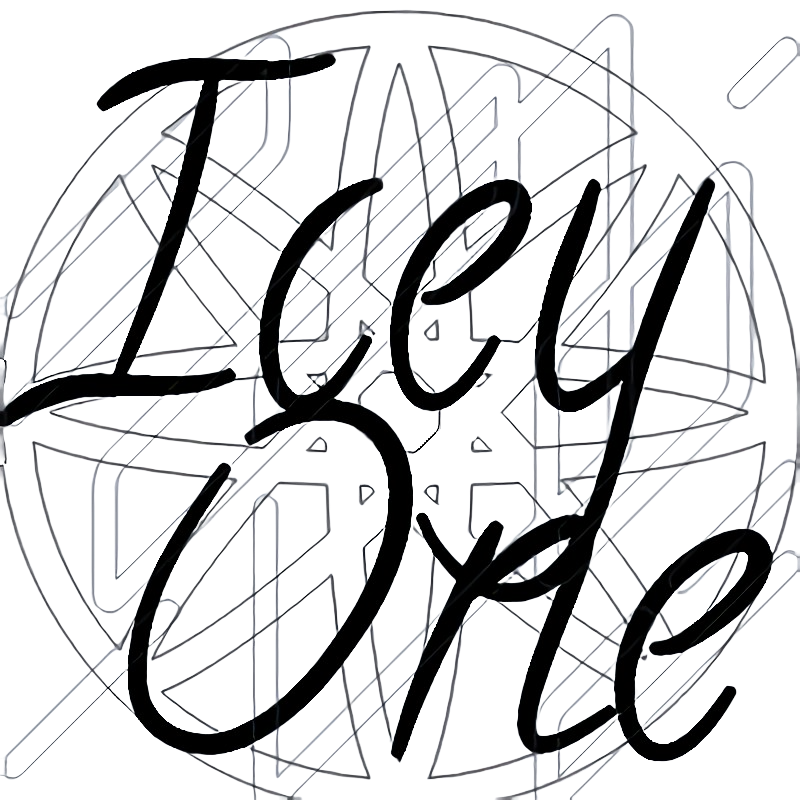
\includegraphics[width=\textwidth]{IceyOne.png}
    \caption{图片测试}
    \label{fig:myphoto}
\end{figure}
\begin{lstlisting}
    \begin{figure}[htbp]
        \centering
        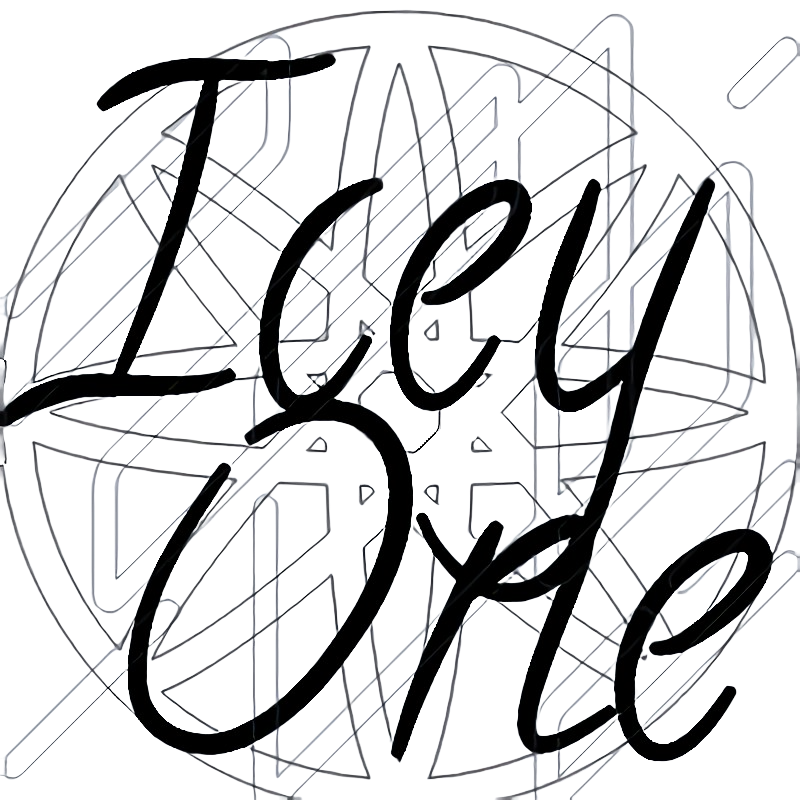
\includegraphics[width=0.10\textwidth]{IceyOne.png}
        \caption{图片测试}
        \label{fig:myphoto}
    \end{figure}
\end{lstlisting}
\subsection{表格测试}
如果对 \LaTeX 不太熟悉, 建议用 \href{https://www.tablesgenerator.com/}{Tables Generator} 或者 \href{https://tableconvert.com/}{Table Convert} 快速生成表格.
\begin{table}[htbp]
    \centering
    \caption{表格测试}
    \label{table:test}
    \begin{tabular}{llll}
        \hline
        Paremater & Markwodn & \LaTeX & Word \\ \hline
        上手难度 & 易 & 易 & 易 \\
        数学排版 & 支持 \LaTeX & 易 & 难 \\
        定制 & 易 & 很难 & 易 \\
        结构化 & 是 & 是 & 否 \\ \hline
    \end{tabular}
\end{table}
\begin{lstlisting}
    \begin{table}[htbp]
        \centering
        \caption{表格测试}
        \label{table:test}
        \begin{tabular}{llll}
            \hline
            Paremater & Markwodn & \LaTeX & Word \\ \hline
            上手难度 & 易 & 易 & 易 \\
            数学排版 & 支持 \LaTeX & 易 & 难 \\
            定制 & 易 & 很难 & 易 \\
            结构化 & 是 & 是 & 否 \\ \hline
        \end{tabular}
    \end{table}
\end{lstlisting} 
%\include{includefile/Chapter4}
%------------ 附录 Appendix ----------%
\appendix
%--------- 参考文献 References --------%
\cleardoublepage\phantomsection
\bibliographystyle{gbt7714-numerical} % 设定引用文献格式

%----------- 使用 Bib 文件 ------%
%\addcontentsline{toc}{chapter}{参考文献}
%\bibliography{references.bib}

%------ 手动添加参考文献------%
\addcontentsline{toc}{chapter}{参考文献}
\begin{thebibliography}{99}
  \bibitem{ref1} 参考文献 1
  \bibitem{ref2} 参考文献 2
  \bibitem{ref3} 参考文献 3
  \bibitem{ref4} 参考文献 4
\end{thebibliography}

\cleardoublepage
\end{document}